The respondents are asked three questions:

\begin{enumerate}
	\item If medical information could be shared electronically between places where a patient receives medical care, how would that affect the privacy and security of medical info?
(Likert scale from 1 to 5, graphically symbolized by stars from left - worst - to right - best)

\item Now how do you think that would affect the quality of medical information?
(as before)

\item In general, how would you rate your overall health?
(Likert scale from 1 to 5, from "Poor" to "Excellent")
\end{enumerate}

\subsection{Standard questionnaire}
The standard questionnaire is modeled to exactly replicate the order in which the three CNSS questions were fielded (see \href{https://www.sri.cornell.edu/sri/files/cnss/2012/CNSS2012questionnaire.pdf#page=19}{CNSS 2012 Questionnaire, page 19}). Respondents first see Question 1 (Figure~\ref{fig:q1})%
\footnote{The images shown are available while building the survey, and represent a simulated webpage typical of the one respondents would be browsing. We did not capture the equivalent pages adapted for mobile devices. For screenshots of users of the ``Google Consumer Surveys'' mobile application, see Appendix.}
, as well as options to choose other surveys fielded by Google Consumer Surveys, and alternate methods to access the content:

\begin{figure}
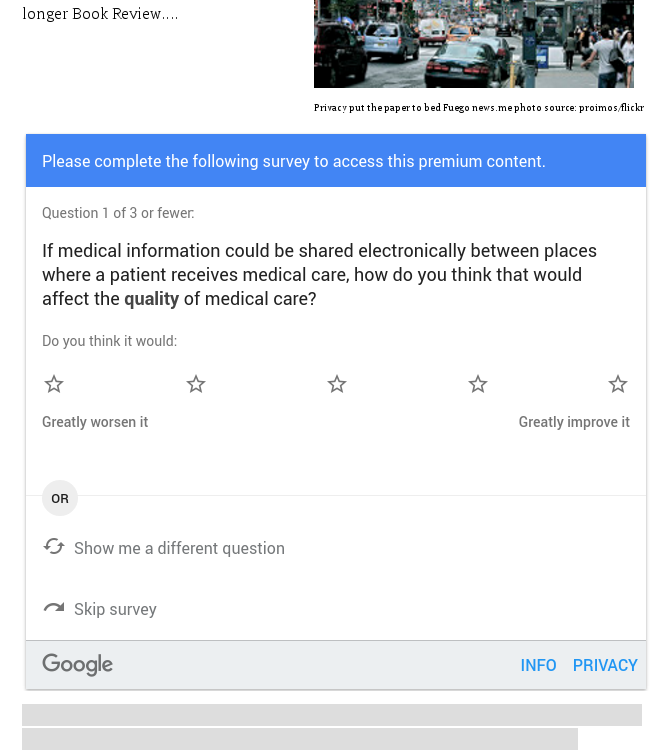
\includegraphics[width=\textwidth]{Selection_351.png}
\caption{\label{fig:q1}Question 1: Quality of Medical Care}
\end{figure}
\begin{figure}
	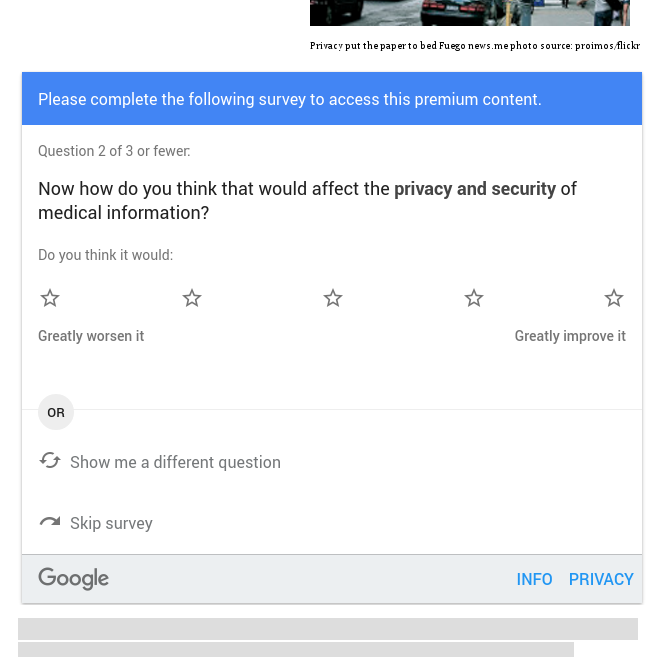
\includegraphics[width=\textwidth]{Selection_352.png}
	\caption{\label{fig:q2}Question 2: Privacy}
\end{figure}
\begin{figure}
	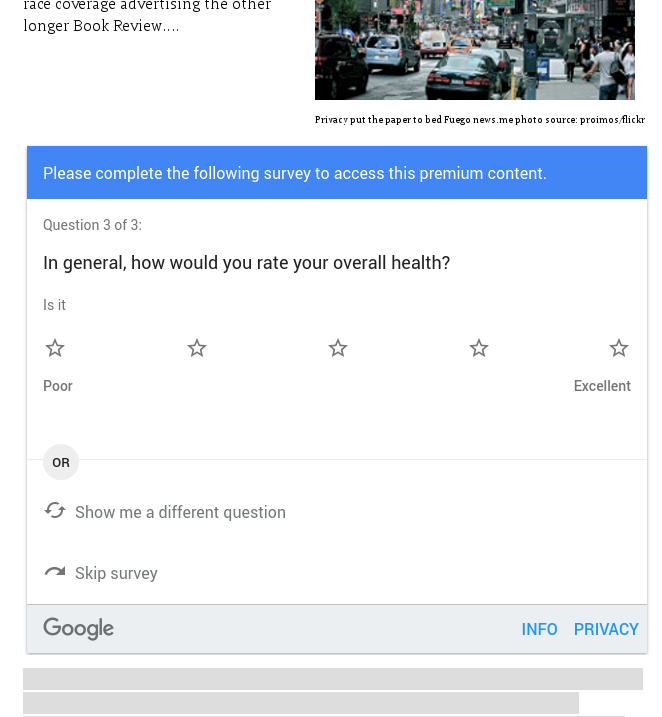
\includegraphics[width=\textwidth]{Selection_353.png}
	\caption{\label{fig:q3}Question 3: Health overall}
\end{figure}

\subsection{Variations}
\subsubsection{Inversion of Q1 and Q2}
The questions are the same as before, but with the order in which opinion on quality and privacy was asked inverted. The changed order appears in the header of the text, but otherwise the questions are unchanged. 

%![Question 1 Questionnaire 2](../data/raw_gcs_2017/Selection_357.png "Question 1")
%![Question 2 Questionnaire 2](../data/raw_gcs_2017/Selection_358.png "Question 2")

Question 3 was exactly the same as before.

\subsubsection{Shortened questionnaire}
For a fraction of the respondents, Q1 or Q2 are randomly dropped. Respondents know this before hand (the total number of questions is indicated to the potential respondent before entering the survey). Figure~\ref{fig:q1dropped} shows the resulting question when Q1 (quality) is dropped, and Figure~\ref{fig:q2dropped} when Q2 (privacy) is dropped. The only difference with respect to Figures~\ref{fig:q1} and~\ref{fig:q2} is the text ``Question 1 of 2'' instead of ``Question 1 of 3 or fewer'', shown below the blue bar.

\begin{figure}
	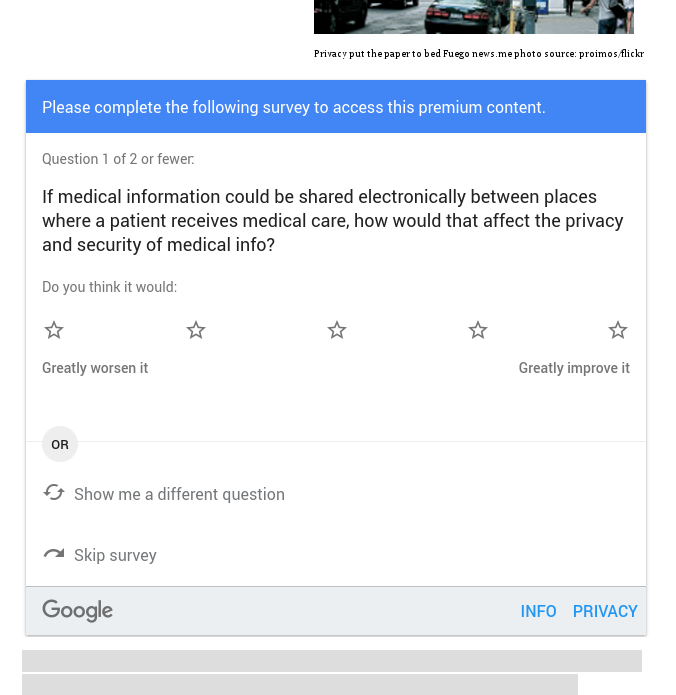
\includegraphics[width=\textwidth]{Selection_354.png}
	\caption{\label{fig:q1dropped}First question when quality (Q1) is dropped}
\end{figure}
\begin{figure}
	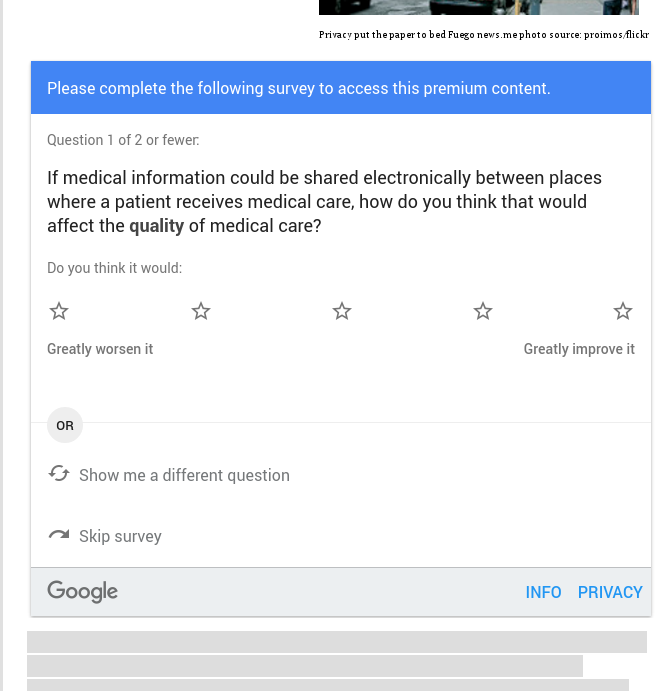
\includegraphics[width=\textwidth]{Selection_356.png}
	\caption{\label{fig:q2dropped}First question when privacy (Q2) is dropped}
\end{figure}
In both cases, the second and final question is the health status question:

\begin{figure}
	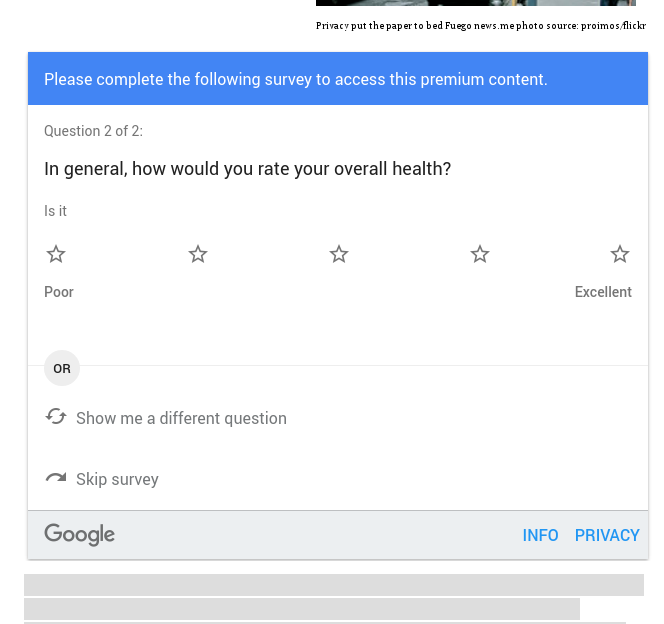
\includegraphics[width=\textwidth]{Selection_355.png}
	\caption{\label{fig:qfinalshort}Question 2 of shortened questionnaire}
\end{figure}
